\begin{frame}{The Standard Model of Particle Physics}
  \framesubtitle{State of the art}

  \begin{columns}
    
    \begin{column}{0.5\textwidth}

      \begin{figure}
        \centering
        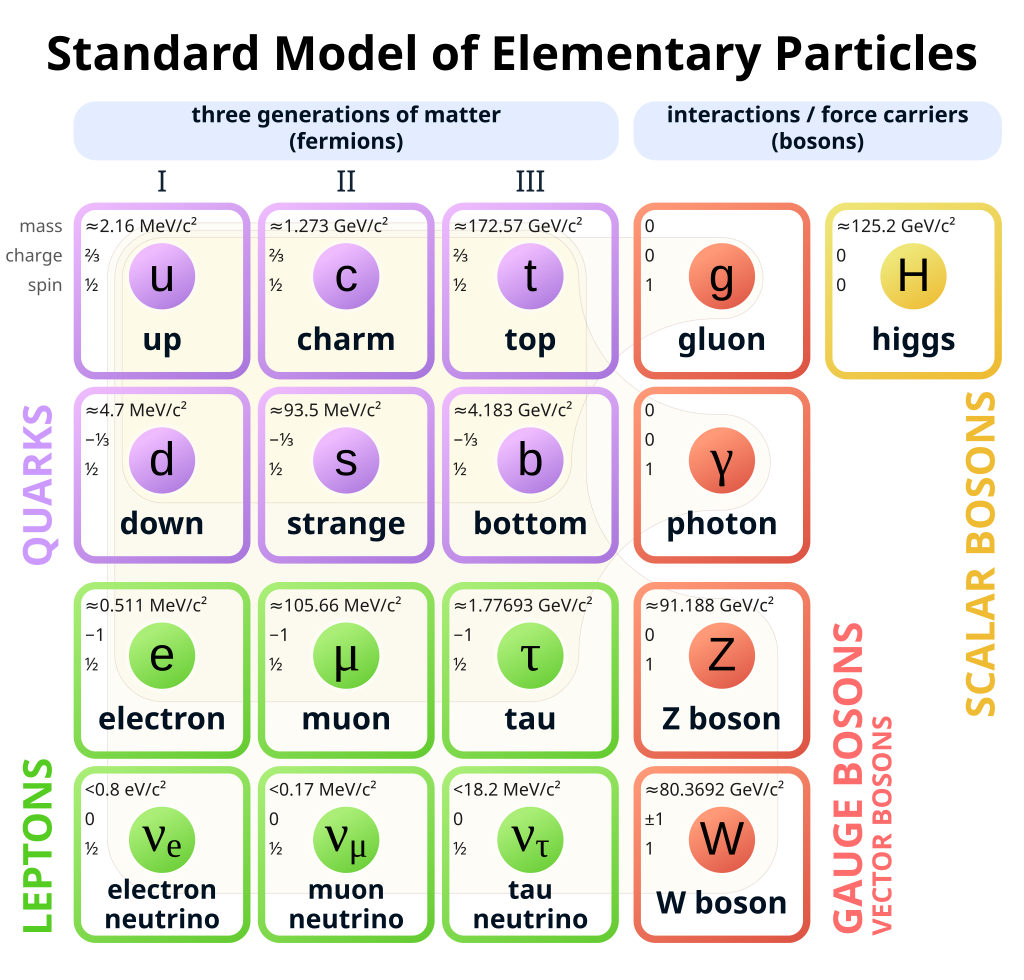
\includegraphics[width = \textwidth]{imgs/standard-model.png}
      \end{figure}

    \end{column}

    

    \begin{column}{0.5 \textwidth}
    \begin{center}
        High energy $\to$ Special Relativity \\
        Small particles $\to$ Quantum Mechanics \\
        $\downarrow$ \\
        Quantum Field Theory \\
        (mathematical framework)
    \end{center}
    
    

      \begin{colorblock}[black]{statalelightgreen}{Evidences for physics beyond the SM}
        \begin{itemize}
          \item Dark matter and dark energy
          \item Matter-antimatter asymmetry
          \item Origin of neutrino masses
        \end{itemize}
      \end{colorblock}

      \vspace{0.5em}


      

    \end{column}

  \end{columns}

\end{frame}

%=======================================================================

\begin{frame} {Collider Physics}
  \framesubtitle{One of the principal methods of research}

   \begin{columns}
  
    \begin{column}{0.5\textwidth}
    \textbf{L}arge \textbf{H}adron \textbf{C}ollider at CERN \\
    Proton beams accelerated to $\sim 13.6 \, \text{TeV}$ \\

      \begin{figure}
        \centering
        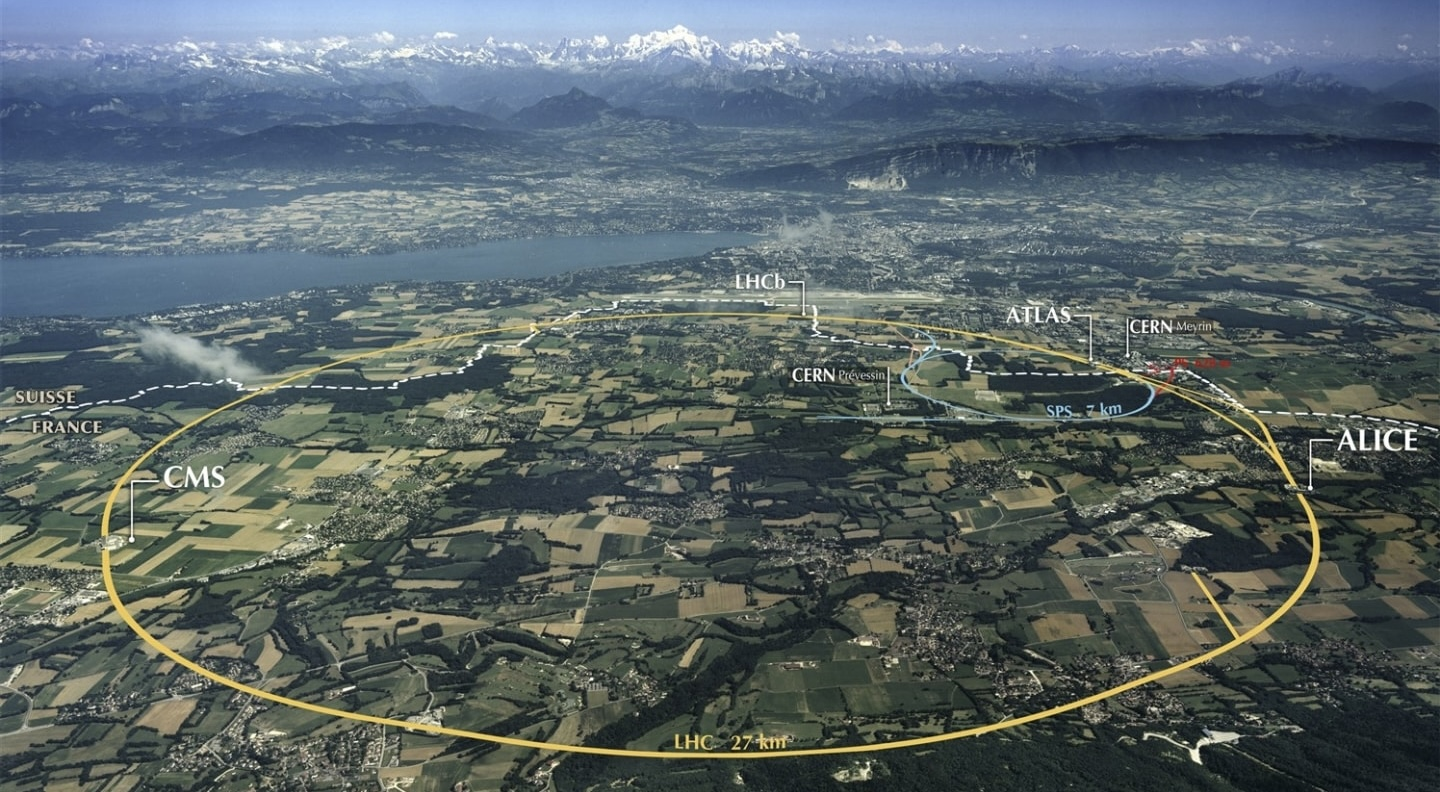
\includegraphics[width=\textwidth]{imgs/lhc.jpeg}
        \caption{ Maximilien Brice/CERN}
      \end{figure}
    \end{column}


    \begin{column}{0.5\textwidth}
        \begin{centering}
            Not sufficient to the discovery of new particles. \\

            \vspace{2.0em}
        Solutions: 
        \vspace{0.8em}
        \begin{itemize}
        \item Increase energy \\$\to$ not feasible or extremely expensive\\ \quad with existing technology
        \end{itemize}
        \end{centering}

        \begin{colorblock}[black]{statalelightgreen}{}
        \begin{itemize}
          \item Increase precision  \\$\to$ both experimental and \textbf{theoretical}
        \end{itemize}
      \end{colorblock}
    
    \end{column}

    \end{columns}
  
\end{frame}


%=======================================================================

\begin{frame} {Quantum Chromodynamics}
  \framesubtitle{Hard scattering processes}

   \begin{columns}

    \begin{column}{0.5\textwidth}

    \vspace{0.5em}
    
        \begin{itemize}
            \item Strong interactions are described by Quantum Chromodynamics (QCD).
            \item Non-Abelian gauge theory, \\$SU(3)$ symmetry group.
            \item The QCD Lagrangian is not analytically solvable.
        \end{itemize}

    \vspace{0.5em}
    \pause
    \begin{colorblock}[black]{statalelightgreen}{Hadron collisions}
        \begin{itemize}
          \item Elastic scattering
          \item Diffractive dissociation
          \item \textcolor{red}{\textbf{Hard scattering}} \\(momentum exchange $\sim 100 \,\text{GeV}$)
        \end{itemize}
      \end{colorblock}
    
  
    \end{column}

    \begin{column}{0.5\textwidth}
        \begin{figure}
        \centering
        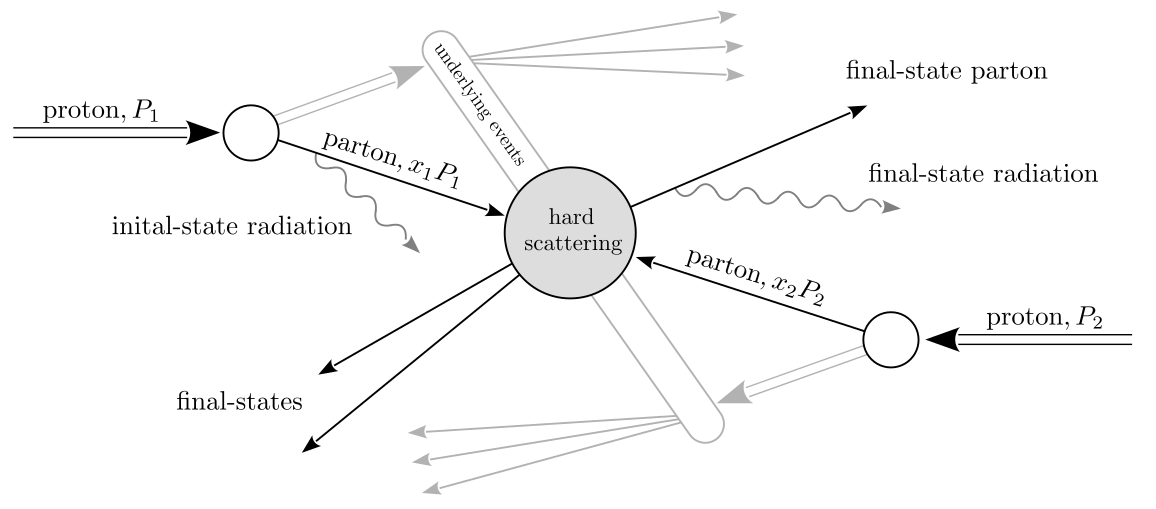
\includegraphics[width=\textwidth]{imgs/hard-scattering.png}
        \caption{Konstantin Asteriadis/KIT}
      \end{figure}

      \textbf{Asymptotic freedom} \\
      Interacting partons can be approximated as being nearly free\\
      $\to$ \textbf{Perturbative description}
    
    \end{column}

    \end{columns}
  
\end{frame}


%=======================================================================

\begin{frame} {The collinear factorization theorem}
  \framesubtitle{A framework for describing hard scattering processes}
    
   \begin{columns}

    \begin{column}{0.6\textwidth}
    Colliding hadrons are treated as \textbf{beams of partons}, carrying a fraction of the hadron's total momentum
    
   \begin{colorblock}[black]{statalelightgreen}{Separation of energy scales}
        \begin{itemize}
          \item SM interactions $Q \sim 100 \text{GeV}-1\text{TeV}$
          \item Hadronic structure $\Lambda_{\mathrm{QCD}}\sim 100\text{MeV}$
        \end{itemize}
      \end{colorblock}
\begin{centering}
    $\to$ \textbf{Decoupling} the motions of partons from proton's dynamics
\end{centering}
    
    \end{column}

    \begin{column}{0.4\textwidth}
       \begin{figure}
        \centering
        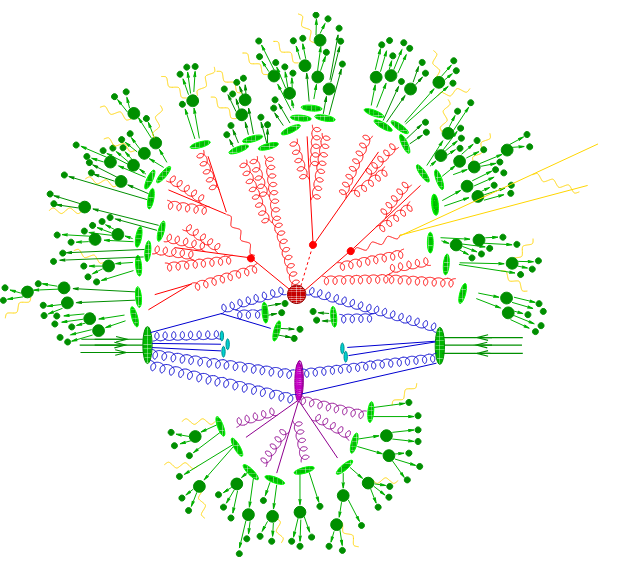
\includegraphics[width=0.8\textwidth]{imgs/hadron-collision.png}
        \caption{Stefan Höche/SLAC National Accelerator Laboratory}
      \end{figure}
    
    \end{column}

    \end{columns}
    \begin{equation*}
    \text{d}\sigma=\sum_{a, b} \int_0^1 \text{d}x_1 \text{d}x_2 f_{a}(x_1, \mu_\text{F}) f_{b}(x_2,\mu_\text{F}) \, \textcolor{red}{\text{d}\hat \sigma_{a,b}(x_1,x_2,\mu_\text{F},\mu_\text{R};\mathcal{O})} \left(1+ \mathcal{O}\left(\frac{\Lambda_{\text{QCD}}}{Q} \right)^n \right), \, n\geq1
    \label{fact-theor}
\end{equation*}
  
\end{frame}


%=======================================================================

\begin{frame} {The partonic cross section}
  \framesubtitle{A perturbative description}
\vspace{1em}
The partonic cross section can be expanded in powers of the strong and the electroweak coupling constants, $\alpha_{\text{S}}$ and $\alpha$
    \begin{equation*}
    \text{d} \hat{\sigma}_{a,b} = \text{d} \hat{\sigma}_{a,b}^{(0,0)} + \textcolor{magenta}{\alpha_s \text{d} \hat{\sigma}_{a,b}^{(1,0)}} + \alpha_s^2 \text{d} \hat{\sigma}_{a,b}^{(2,0)} + \alpha_s^3 \text{d} \hat{\sigma}_{a,b}^{(3,0)} + \alpha \text{d} \hat{\sigma}_{a,b}^{(0,1)} + \alpha \alpha_s \text{d} \hat{\sigma}_{a,b}^{(1,1)} + \dots 
    \end{equation*}

    \begin{columns}

    \begin{column}{0.6\textwidth}
    \begin{colorblock}[black]{statalelightgreen}{We focus on  NLO QCD corrections}
    \begin{center}
        Account for short distance, high-energy effects
    \end{center}
      \end{colorblock}   
    
    \end{column}

    \begin{column}{0.4\textwidth}
    \\
    They consist of three terms 
    \begin{equation*}
    \textcolor{magenta}{\mathrm{d} \hat{\sigma}_{a,b}^{\mathrm{NLO}}} = \textcolor{red}{\mathrm{d} \hat{\sigma}_{a,b}^{\mathrm{R}}} + \textcolor{blue}{\mathrm{d} \hat{\sigma}_{a,b}^{\mathrm{V}}} + \mathrm{d} \hat{\sigma}_{a,b}^{\mathrm{pdf}}
    \end{equation*}       
    
    \end{column}

    \end{columns}
    \begin{figure}
        \centering
        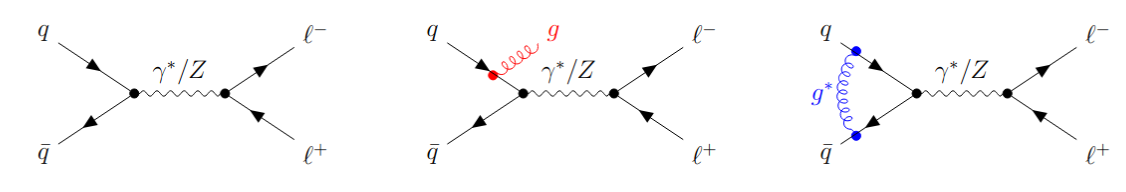
\includegraphics[width=0.8\textwidth]{imgs/real-and-virtual.png}
      \end{figure}    
\end{frame}




%=======================================================================

\begin{frame} {UV and IR divergences}
  \framesubtitle{A considerable obstacle}
  \vspace{1em}
  The treatment of real and virtual corrections is \textbf{non-trivial} \\
  \vspace{1em}
  \textcolor{maincolor}{\textcircled{1}} \textbf{Ultraviolet} (UV) singularities in virtual contributions \\
  \quad $\to$ Renormalization

    \begin{colorblock}[black]{statalelightgreen}{}
        \textcolor{maincolor}{\textcircled{2}} \textbf{Infrared} (IR) singularities in both real and virtual contributions \\
    \quad $\to$ Low-momentum (\textcolor{red}{soft}) and small-angle (\textcolor{blue}{collinear}) kinematic regions
      \end{colorblock}
    
\begin{equation*}
  \begin{tikzpicture}[baseline = (r.base)]
    \begin{feynman}[inline = (r.base)]
      \vertex (a);
      \vertex[right = 2cm of a, dot] (b) {};
      \vertex[right = 2cm of b, circle, draw, fill=lightgray,  minimum size = 1.2cm] (c) {};

      \vertex[above = 1cm of b] (d);
      \vertex[right = 1.5cm of d] (e);

      \vertex[below = 0.25cm of b] (r);

      \diagram* {
	    (a) -- [fermion, momentum' = \(p_i\)] (b),
	    (b) -- [fermion, momentum' = \(p_i - p_\um\)] (c),

	    (b) -- [gluon, momentum = \(p_\um\)] (e),
        };
    \end{feynman}
  \end{tikzpicture}
  \, \sim \,
  \frac{1}{(p_i - p_\um)^2} = \frac{1}{2 E_i E_\um \left( 1 - \cos \theta_{i \um} \right)} \quad
  \xrightarrow[\textcolor{red}{E_\um}, \textcolor{blue}{\theta_{i \um}} \to 0 ]{} \quad \infty \,
\end{equation*}

\end{frame}


%=======================================================================

\begin{frame} {UV and IR divergences}
  \framesubtitle{Dimensional regularization and pole cancellation}

  \begin{columns}

    \begin{column}{0.4\textwidth}
    \begin{colorblock}[black]{statalelightgreen}{Dimensional regularization}
        \begin{equation*}
            d=4-2\epsilon \qquad \epsilon \in \mathbb{C} \, , \mathrm{Re}(\epsilon)<0
        \end{equation*}
      \end{colorblock}
    \end{column}

    \begin{column}{0.6\textwidth}
    Divergences appear as poles in $1/\epsilon$ \\
    \begin{itemize}
        \item Virtual $\to$ explicit
        \item Real $\to$ phase space integration needed \textcolor{red}{\textcircled{1}}
    \end{itemize}
    \end{column}
    \end{columns}

    \vspace{1.5em}

    \begin{itemize}
        \item Singularities signal the presence of long-distance (low-energy) effects
        \item The division into real and virtual terms is therefore a computational tool
    \end{itemize}

    \vspace{1.em}
\pause
    \begin{colorblock}[black]{statalelightgreen}{Bloch-Nordsieck and Kinoshita-Lee-Nauenberg theorems}
            Infrared divergences are \textbf{guaranteed} to cancel when we sum real and virtual corrections
      \end{colorblock}

      \begin{itemize}
        \item \textbf{Mismatch} in the dimensionality of the integration domains \textcolor{red}{\textcircled{2}}
    \end{itemize}
\end{frame}

%=======================================================================

\begin{frame} {IR divergences}
 \framesubtitle{Subtraction scheme}
Insights \\
\begin{itemize}
    \item \textbf{Factorization} of the amplitudes in the soft and collinear limits 
    \item Real emissions are \textbf{unresolved} in singular kinematics regions
\end{itemize}
 \vspace{0.5em}
 We adopt a \textbf{subtraction method}
\begin{equation*}
    2s_{a,b} \mathrm{d} \hat{\sigma}_{a,b}^{\mathrm{R}} = \int [\mathrm{d}p_{\um}] F_{\mathrm{LM}} (\um)=  \textcolor{red}{\int [\mathrm{d}p_{\um}] (F_{\mathrm{LM}}(\um) - \mathcal{S})}  + \textcolor{blue}{\int [\mathrm{d}p_{\um}] \mathcal{S}}
    \label{subtraction-flm}
\end{equation*}
\textcolor{blue}{$\to$} Describes the singular behaviour of the amplitude\\ 
\textcolor{red}{$\to$} Singular behaviour removed: numerical integration with Monte Carlo methods \\

\pause

  \begin{columns}

    \begin{column}{0.50\textwidth}
 \begin{colorblock}[black]{statalelightgreen}{}
\begin{center}
    Restricting the integration region to the \\\textbf{minimal necessary volume} is crucial for improving the efficiency of the computation
\end{center}
\end{colorblock}
    \end{column}

    \begin{column}{0.50\textwidth}
    \begin{center}
        Current calculations require $\sim 106$ CPUh\textsuperscript{[1]} \\
        $\to$ Further refinements needed for NNLO calculations 
    \end{center}
    \end{column}
    \end{columns}

\vspace{0.3em}
    {\tiny
[1] Czakon et al., SciPost Phys. 11, 001 (2021), Tour de force in Quantum Chromodynamics
}





\end{frame}

%=======================================================================
\begin{frame} {NSC Subtraction Scheme}
   \framesubtitle{Sequential extraction of singularities}
\begin{columns}
\begin{column}{0.50\textwidth}
  \begin{center}
    FKS (Frixione, Kunszt, Signer) constructs $S$ from the soft and collinear limits
  \end{center}

    \end{column}

    \begin{column}{0.50\textwidth}
    \begin{equation*}
    S_i A := \lim_{E_i \to 0} A \, , \qquad C_{ij}A := \lim_{\rho_{ij}\to 0}A 
\end{equation*}
    \end{column}
\end{columns}
 \vspace{1.5em}

The singularities are isolated and extracted \textbf{sequentially} in a nested manner
\begin{equation*}
  \langle \Delta^{(\um)}F_{\mathrm{LM}}(\um) \rangle = \textcolor{red}{\langle S_{\um}F_{\mathrm{LM}}(\um) \rangle} + \sum_{i=1}^{N_p} \textcolor{blue}{\langle \bar{S}_{\um}C_{i\um} \Delta^{(\um)} F_{\mathrm{LM}}(\um) \rangle} + \textcolor{orange}{\langle \bar{S}_{\um} \bar{C}_{i\um} \Delta^{(\um)} \omega^{\um i} F_{\mathrm{LM}}(\um) \rangle}
\end{equation*}

\begin{columns}
\begin{column}{0.50\textwidth}
    $\textcolor{red}{\to}$ First, we remove the soft singularities\\
$\textcolor{blue}{\to}$ Then, the collinear and soft-collinear ones\\
$\textcolor{orange}{\to}$ \textbf{Completely finite} term, can be integrated\\ \, \quad in four dimensions

    \end{column}

    \begin{column}{0.50\textwidth}
    \begin{itemize}
      \item $\bar{S}_\um= \mathbb{1} - S_\um$, $\bar{ C}_\um= \mathbb{1} - C_\um$
      \item $\omega^{\um i}$ in order to treat one collinear singularity at a time
      \item $\Delta^{(\um)}$ to select the unresolved parton
    \end{itemize}
    \end{column}
\end{columns}


\end{frame}
%=======================================================================

\begin{frame} {NSC Subtraction Scheme}
  \framesubtitle{The soft term}
We integrate over the phase space of the unresolved parton $\um$ 
\begin{equation*}
  \langle S_\um F_{\mathrm{LM}} (\um) \rangle = \int \mathrm{d}E_\um E_\um^{d-5} \, \theta(E_\um < E_{\mathrm{max}})  \int \frac{\mathrm{d}\Omega_{d-1}}{2 (2 \pi)^{d-1}} (-g_{s,b}^2) \sum_{(i \neq j)}^{N_p} \frac{\rho_{ij}}{\rho_{im}\rho_{jm}} (\vec{T}_i \cdot \vec{T}_j) F_{\mathrm{LM}} \, ,
\end{equation*}

\pause
We introduce the parameter $\theta_s$, which limits the energy of unresolved partons
\begin{equation*}
  \langle S_\um^{\textcolor{red}{\theta_s}} F_{\mathrm{LM}} (\um) \rangle = \int \mathrm{d}E_\um E_\um^{d-5} \, \theta(E_\um < \textcolor{red}{\theta_s} E_{\mathrm{max}})  \int \frac{\mathrm{d}\Omega_{d-1}}{2 (2 \pi)^{d-1}} (-g_{s,b}^2) \sum_{(i \neq j)}^{N_p} \frac{\rho_{ij}}{\rho_{im}\rho_{jm}} (\vec{T}_i \cdot \vec{T}_j) F_{\mathrm{LM}} 
\end{equation*}
\pause
And we obtain \qquad \qquad \quad $\langle S_\um^{\textcolor{red}{\theta_s}} F_\mathrm{LM}(\um) \rangle = [\alpha_s] \langle I_{\mathrm{S}}\cdot F_{\mathrm{LM}} \rangle$
\begin{colorblock}[black]{statalelightgreen}{}
    \begin{equation*}
  I_{\mathrm{S}} (\epsilon, \theta_s)= -\frac{1}{\epsilon^2} \left(\frac{2E_{\mathrm{max}}}{\mu}\right)^{-2\epsilon} \, \textcolor{red}{\theta_s^{-2\epsilon}} \, \sum_{i \neq j }^{N_p} \eta_{ij}^{-\epsilon} \, K_{ij} \, \left( \vec{T}_i \cdot \vec{T}_j\right)
        \end{equation*}
      \end{colorblock}


\end{frame}

%=======================================================================

\begin{frame} {NSC Subtraction Scheme}
  \framesubtitle{The collinear term - initial state}
We integrate over the phase space of the unresolved parton $\um$ 
\begin{equation*}
  \begin{aligned}
  \int [\mathrm{d}p_\um]\, C_{a\um}  F_{\mathrm{LM}} (\um) &= \frac{1}{8\pi^2} \frac{(4\pi)^{\epsilon}}{\Gamma(1-\epsilon)} 2^{-2\epsilon} \int_0^{1} \mathrm{d}\eta_{a\um} (\eta_{a\um}(1-\eta_{a\um}))^{-\epsilon} \times \\
  & \times \int_{0}^{E_{\mathrm{max}}} \mathrm{d}E_\um E_\um^{1-2\epsilon} \frac{g_{s,b}^2}{(1-z)E_a^2 \eta_{a\um}} \frac{P_{f_{[a\um]}f_a}(z)}{z} F_{\mathrm{LM}} (z \cdot a) \, ,
  \end{aligned}
\end{equation*}

\pause
We introduce the parameter $\theta_a$, which controls the angular separation of unresolved partons
\begin{equation*}
  \begin{aligned}
  \int [\mathrm{d}p_\um]\, C_{a\um}^{\textcolor{blue}{\theta_a}}  F_{\mathrm{LM}} (\um) &= \frac{1}{8\pi^2} \frac{(4\pi)^{\epsilon}}{\Gamma(1-\epsilon)} 2^{-2\epsilon} \int_0^{\textcolor{blue}{\theta_a}} \mathrm{d}\eta_{a\um} (\eta_{a\um}(1-\eta_{a\um}))^{-\epsilon} \times \\
  & \times \int_{0}^{E_{\mathrm{max}}} \mathrm{d}E_\um E_\um^{1-2\epsilon} \frac{g_{s,b}^2}{(1-z)E_a^2 \eta_{a\um}} \frac{P_{f_{[a\um]}f_a}(z)}{z} F_{\mathrm{LM}} (z \cdot a) \, ,
  \end{aligned}
\end{equation*}
\end{frame}

%=======================================================================

\begin{frame} {NSC Subtraction Scheme}
  \framesubtitle{The collinear term - final state}
We integrate over the phase space of the unresolved parton $\um$ 

  \begin{align*}
  \int [\mathrm{d}p_i] \int [\mathrm{d}p_\um] \, C_{i\um} \Delta^{(\um)} F_{\mathrm{LM}} 
  &= \int \frac{\mathrm{d}\Omega^{d-2}}{2(2\pi)^{d-1}} 2^{-2\epsilon} \int_0^1 \frac{\mathrm{d}\eta_{i\um}}{(\eta_{i\um}(1-\eta_{i\um}))^{\epsilon}} \nonumber \\
  &\quad \times \int [\mathrm{d}\Omega_i] \int \mathrm{d}E_\um E_\um^{1-2\epsilon} \int \mathrm{d}E_i E_i^{1-2\epsilon} 
  \frac{g_{s,b}^2 P_{f_{[i\um]}f_i} F_{\mathrm{LM}} (i\um) }{(1-z) E_{i\um}^{2}\eta_{i\um}} .
    \end{align*}


\pause
We introduce the parameter $\theta_i$, which controls the angular separation of unresolved partons
\begin{equation*}
  \begin{aligned}
    \int [\mathrm{d}p_i] \int [\mathrm{d}p_\um] \, C_{i\um}^{\textcolor{blue}{\theta_i}} \Delta^{(\um)} F_{\mathrm{LM}} &= \int \frac{\mathrm{d}\Omega^{d-2}}{2(2\pi)^{d-1}} 2^{-2\epsilon} \int_0^{\textcolor{blue}{\theta_i}} \frac{\mathrm{d}\eta_{i\um}}{(\eta_{i\um}(1-\eta_{i\um}))^{\epsilon}} \nonumber \\
    &\quad \times \int [\mathrm{d}\Omega_i] \int \mathrm{d}E_\um E_\um^{1-2\epsilon} \int \mathrm{d}E_i E_i^{1-2\epsilon} \frac{g_{s,b}^2 \,  P_{f_{[i\um]}f_i} \, F_{\mathrm{LM}} (i\um) }{(1-z) E_{i\um}^{2}\eta_{i\um}} \, .
  \end{aligned}
\end{equation*}
\end{frame}

%=======================================================================

\begin{frame} {NSC Subtraction Scheme}
  \framesubtitle{The collinear term}
\begin{equation*}
  \begin{aligned}
    \sum_{i \in \mathcal{H}_f} \langle C_{i\mathfrak{m}}^{\textcolor{blue}{\theta_i}} \bar{S}_{\mathfrak{m}}^{\textcolor{red}{\theta_s}} \Delta^{\mathfrak{m}} F_{\mathrm{LM}}(\mathfrak{m})\rangle &= [\alpha_s]\langle I_{\mathrm{C}}(\epsilon, \theta_s, \theta_i) \cdot F_{\mathrm{LM}} \rangle \\
    & + [\alpha_s] \bigl< [\mathrm{d}\eta_{a\um \, \theta_a}] \left(\frac{2E_a}{\mu}\right)^{-2\epsilon} \int_{0}^{1} \mathrm{d}z \, \left[\hat{P}_{aa}^{(0)}-\epsilon \mathcal{P}_{aa}^{\mathrm{fin}}\right] \frac{1}{z} \, F_{\mathrm{LM}}(z\cdot a) \bigr> \\
    & + [\alpha_s] \bigl< [\mathrm{d}\eta_{b\um \, \theta_b}] \left(\frac{2E_b}{\mu}\right)^{-2\epsilon} \int_{0}^{1} \mathrm{d}z \, \left[\hat{P}_{bb}^{(0)}-\epsilon \mathcal{P}_{bb}^{\mathrm{fin}}\right] \frac{1}{z} \, F_{\mathrm{LM}}(z\cdot b) \bigr> \, ,
  \end{aligned}
\end{equation*}
\begin{colorblock}[black]{statalelightgreen}{}
  \begin{equation*}
  \begin{aligned}
    I_{\mathrm{C}} (\epsilon, \theta_s, \theta_i) = &\sum_{i \in \mathcal{H}} \biggl( \frac{1}{\epsilon}\, \left(\, \gamma_i+  2 \,L_i^{\textcolor{red}{\theta_s}} \,\vec{T}_i^2 \right) - 2 \log{\left(\frac{2E_i}{\mu}\right)}\, \gamma_i  - 4 \, \vec{T}_q^2 \, L_i^{\textcolor{red}{\theta_s}} \log{\left(\frac{2E_i}{\mu}\right)} \\
    & - \log{(\textcolor{blue}{\theta_i})} \, \gamma_i - 2 \log{(\textcolor{blue}{\theta_i})} \, \vec{T}_i^2 \, L_i^{\textcolor{red}{\theta_s}} \biggr) 
    \label{green}
  \end{aligned}
\end{equation*}
      \end{colorblock}

\end{frame}
%=======================================================================

\begin{frame} {Cancellation of poles}
  \framesubtitle{Unaffected by the $\theta$-parameters}
\begin{equation*}
  \begin{aligned}
  \textcolor{black}{I_{\mathrm{S}} (\epsilon, \theta_s)} &= \frac{1}{\epsilon^2}\sum_{i=1}^{N_p} T_i^2 + \textcolor{orange}{\frac{1}{\epsilon}}\left[-\sum_{i=1}^{N_p}  \left( \textcolor{orange}{2{L_i}^{\textcolor{red}{\theta_s}}} + 2 \log{\left(\frac{2 E_i}{\mu} \right) } \right) \textcolor{orange}{\vec{T}_i^2} - \sum_{i\neq j}^{N_p} f_1(\eta_{ij}) (\vec{T}_i \cdot \vec{T}_j) \right]  \\
  &  + \sum_{i=1}^{N_p} 2 \log^2{\left(\frac{2 E_{\mathrm{max}}\textcolor{red}{\theta_s}}{\mu} \right)}\vec{T}_i^2 - \sum_{i\neq j}^{N_p} \left[ f_2 \left(2 E_{\mathrm{max}}\textcolor{red}{\theta_s}\right) f_1(\eta_{ij}) + K_{ij}^{(2)}\right] (\vec{T}_i \cdot \vec{T}_j) + \mathcal{O}(\epsilon)
  \end{aligned}
  \label{pink}
\end{equation*}
\pause
  \begin{equation*}
  \begin{aligned}
    \textcolor{black}{I_{\mathrm{C}} (\epsilon, \theta_s, \theta_i)} = &\sum_{i \in \mathcal{H}} \biggl( \textcolor{orange}{\frac{1}{\epsilon}}\, \left(\, \gamma_i+  \textcolor{orange}{2 \,L_i^{\textcolor{red}{\theta_s}} \,\vec{T}_i^2} \right) - 2 \log{\left(\frac{2E_i}{\mu}\right)}\, \gamma_i  - 4 \, \vec{T}_q^2 \, L_i^{\textcolor{red}{\theta_s}} \log{\left(\frac{2E_i}{\mu}\right)} \\
    & - \log{(\textcolor{blue}{\theta_i})} \, \gamma_i - 2 \log{(\textcolor{blue}{\theta_i})} \, \vec{T}_i^2 \, L_i^{\textcolor{red}{\theta_s}} \biggr) 
    \label{green}
  \end{aligned}
\end{equation*}
\pause
The parameter \textcolor{red}{$\theta_s$} appears only as a residue of the \textcolor{orange}{$1/\epsilon$} pole, but its dependence cancels out when summing $I_{\mathrm{S}} + I_{\mathrm{V}}$; both parameters, \textcolor{blue}{$\theta_i$} and \textcolor{red}{$\theta_s$}, appear in finite terms 

\end{frame}

%=======================================================================

\begin{frame} {Cancellation of poles}
  \framesubtitle{Results and future outlook}
The $1/\epsilon^2$ pole cancels summing $I_{\mathrm{S}}+I_{\mathrm{V}}$, the $1/\epsilon$ poles cancel summing $I_{\mathrm{S}}+I_{\mathrm{C}}+I_{\mathrm{V}}$, leaving a finite $I_{\mathrm{T}}^{\mathrm{fin}}=I_{\mathrm{S}}+I_{\mathrm{C}}+I_{\mathrm{V}}$ operator
 \begin{equation*}
 \begin{aligned}
     I_{\mathrm{T}}^{\mathrm{fin}}(\theta_s,\theta_i) & = \sum_{i=1}^{N_p} \biggl(2 \log^2{\left(\frac{2 E_{\mathrm{max}}\textcolor{red}{\theta_s}}{\mu} \right)}\vec{T}_i^2  - 2 \log{\left(\frac{2E_i}{\mu}\right)}\, \gamma_i - 4 \, \vec{T}_q^2 \, L_i^{\textcolor{red}{\theta_s}} \log{\left(\frac{2E_i}{\mu}\right)} - \log{(\textcolor{blue}{\theta_i})} \, \gamma_i \\
     & - 2 \log{(\textcolor{blue}{\theta_i})} \, \vec{T}_i^2 \, L_i^{\textcolor{red}{\theta_s}} \biggr) - \sum_{i\neq j}^{N_p} \left[ f_2 \left(2 E_{\mathrm{max}}\textcolor{red}{\theta_s}\right) f_1(\eta_{ij}) + K_{ij}^{(2)}\right] (\vec{T}_i \cdot \vec{T}_j) + I_{\mathrm{V}}^{\mathrm{fin}} +\mathcal{O}(\epsilon)
 \end{aligned}
 \end{equation*}
Thus the NLO QCD correction reads
\begin{equation*}
    2s_{a,b} \mathrm{d}\hat{\sigma}_{a,b}^{\mathrm{NLO}} = 2s_{a,b} \mathrm{d}\hat{\sigma}_{a,b}^{\mathrm{NLO, fin}} + [\alpha_s] \langle I_{\mathrm{T}}\cdot F_{\mathrm{LM}} \rangle + [\alpha_s]\left[\langle \mathcal{P}_{aa}^{\mathrm{NLO, \theta_a}}\otimes F_{\mathrm{LM}}\rangle+\langle F_{\mathrm{LM}}\otimes \mathcal{P}_{aa}^{\mathrm{NLO, \theta_b}}\rangle \right]
\end{equation*}

\end{frame}

%=======================================================================

\definecolor{iceblue}{RGB}{200, 233, 245}          % Azzurro ghiacci

\begin{frame} {Conclusion}
  \framesubtitle{Results and future outlook}

\begin{columns}
\begin{column}{0.60\textwidth}
    \begin{colorblock}[black]{statalelightgreen}{We have shown that}
  \begin{itemize}
    \item The $\theta$ parameters contribute only to $I_\mathrm{S}$ and $I_\mathrm{C}$, while leaving the pole cancellation unaffected
    \item They appear in the finite parts of $I_\mathrm{T}$ and the regularized amplitude
\end{itemize}
      \end{colorblock}

    \end{column}

    \begin{column}{0.40\textwidth}
    The physical result obtained by summing the finite remainders must be independent of $\theta_s$ and $\theta_i$
    $\to$ \textbf{Powerful consistency check}
    \end{column}
\end{columns}

 \vspace{1.5em}
\begin{colorblock}[black]{iceblue}{Future Developments}
  \begin{itemize}
    \item Numerical analysis of how $\theta_s$ and $\theta_i$ variations affect scattering processes
    \item Extension to NNLO and application to more complex physical scenarios
  \end{itemize}
\end{colorblock}

\end{frame}
